% Standalone TikZ figure: predicted similarity graph over fragments.
%
% This file contains only the \begin{tikzpicture} ... \end{tikzpicture} block,
% so it can be \input{} into any host document that loads tikz. To preview as
% a standalone PDF, compile fig_similarity_graph_standalone.tex.

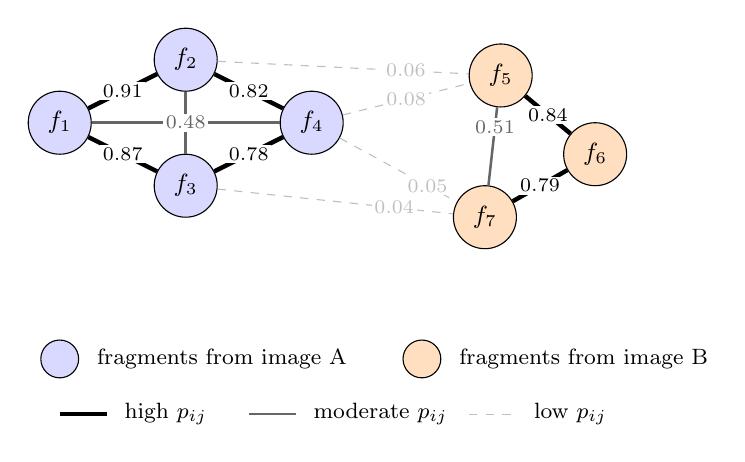
\begin{tikzpicture}[
    node/.style    = {circle, draw, minimum size=8mm, inner sep=0pt, font=\small},
    src1/.style    = {node, fill=blue!15},
    src2/.style    = {node, fill=orange!25},
    edge/.style    = {-, line width=0.6pt},
    strong/.style  = {edge, color=black, line width=1.6pt},
    medium/.style  = {edge, color=black!60, line width=0.9pt},
    weak/.style    = {edge, color=black!25, line width=0.4pt, dashed},
    weight/.style  = {font=\scriptsize, fill=white, inner sep=1pt},
]

% --- nodes: 4 fragments from image A (blue), 3 from image B (orange) ---
\node[src1] (a1) at (0, 2)         {$f_1$};
\node[src1] (a2) at (1.6, 2.8)     {$f_2$};
\node[src1] (a3) at (1.6, 1.2)     {$f_3$};
\node[src1] (a4) at (3.2, 2)       {$f_4$};

\node[src2] (b1) at (5.6, 2.6)     {$f_5$};
\node[src2] (b2) at (6.8, 1.6)     {$f_6$};
\node[src2] (b3) at (5.4, 0.8)     {$f_7$};

% --- intra-A edges (high probability, drawn strong) ---
\draw[strong] (a1) -- (a2) node[weight, midway] {$0.91$};
\draw[strong] (a1) -- (a3) node[weight, midway] {$0.87$};
\draw[strong] (a2) -- (a4) node[weight, midway] {$0.82$};
\draw[strong] (a3) -- (a4) node[weight, midway] {$0.78$};
\draw[medium] (a1) -- (a4) node[weight, midway] {$0.55$};
\draw[medium] (a2) -- (a3) node[weight, midway] {$0.48$};

% --- intra-B edges ---
\draw[strong] (b1) -- (b2) node[weight, midway] {$0.84$};
\draw[strong] (b2) -- (b3) node[weight, midway] {$0.79$};
\draw[medium] (b1) -- (b3) node[weight, near start] {$0.51$};

% --- cross edges (low probability, weak/dashed) ---
\draw[weak] (a4) -- (b1) node[weight, midway] {$0.08$};
\draw[weak] (a4) -- (b3) node[weight, near end] {$0.05$};
\draw[weak] (a2) -- (b1) node[weight, near end] {$0.06$};
\draw[weak] (a3) -- (b3) node[weight, near end] {$0.04$};

% --- legend ---
\begin{scope}[shift={(0, -1.0)}]
    \node[src1, scale=0.6] (lg1) at (0, 0) {};
    \node[anchor=west, font=\footnotesize] at (0.35, 0) {fragments from image A};

    \node[src2, scale=0.6] (lg2) at (4.6, 0) {};
    \node[anchor=west, font=\footnotesize] at (4.95, 0) {fragments from image B};
\end{scope}

\begin{scope}[shift={(0, -1.7)}]
    \draw[strong] (0, 0) -- (0.6, 0);
    \node[anchor=west, font=\footnotesize] at (0.7, 0) {high $p_{ij}$};

    \draw[medium] (2.4, 0) -- (3.0, 0);
    \node[anchor=west, font=\footnotesize] at (3.1, 0) {moderate $p_{ij}$};

    \draw[weak] (5.2, 0) -- (5.8, 0);
    \node[anchor=west, font=\footnotesize] at (5.9, 0) {low $p_{ij}$};
\end{scope}

\end{tikzpicture}
